\documentclass[tikz,border=5mm]{standalone}
\usetikzlibrary{arrows.meta, decorations.pathreplacing}

\begin{document}
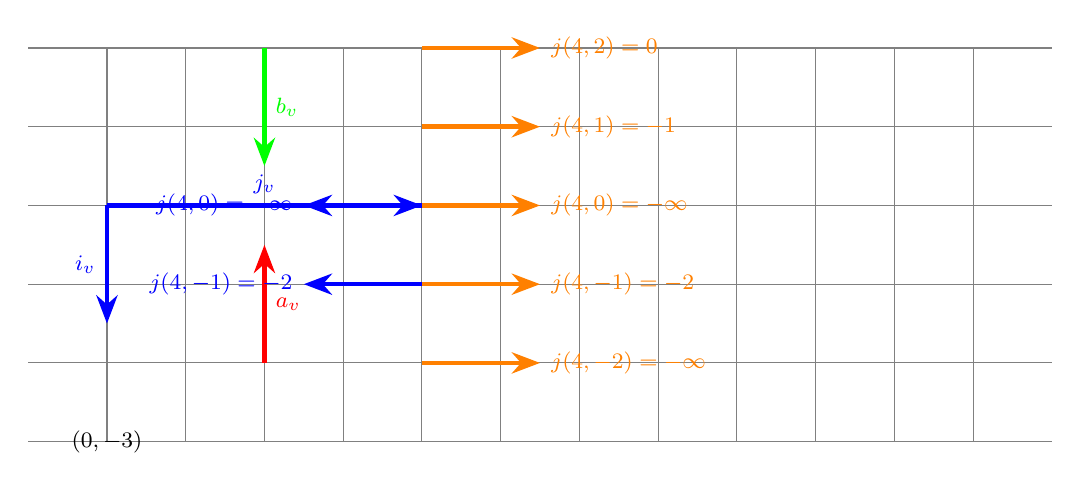
\begin{tikzpicture}[
    >=Stealth,
    every node/.append style={font=\footnotesize},
    axis/.style={help lines, black!50, thin},
    arrow/.style={ultra thick, ->, #1},
]

% Draw coordinate grid and axes
\foreach \y in {-3,...,2}
    \draw[axis] (-1,\y) -- (12,\y);
\foreach \x in {0,1,...,11}
    \draw[axis] (\x,-3) -- (\x,2);

% Draw i_v, j_v, a_v, b_v arrows
\coordinate (i_v) at (0,0);
\coordinate (j_v) at (4,0);
\coordinate (a_v) at (2,-2);
\coordinate (b_v) at (2,2);

\draw[arrow={blue}] (i_v) -- node[above]{$j_{v}$} (j_v);
\draw[arrow={blue}] (i_v) -- node[left]{$i_{v}$}++(-90:1.5) coordinate(i_v_bot);
\draw[arrow={red}] (a_v) -- node[right]{$a_{v}$}++(90:1.5) coordinate(a_v_top);
\draw[arrow={green}] (b_v) -- node[right]{$b_{v}$}++(-90:1.5) coordinate(b_v_bot);

% Draw vertical lines for j(4,k) labels
\foreach \k/\label in {
    2/{j(4,2)=0},
    1/{j(4,1)=-1},
    0/{j(4,0)=-\infty},
    -1/{j(4,-1)=-2},
    -2/{j(4,-2)=-\infty}}
{
    \draw[arrow={orange}] (4,\k) -- ++(1.5,0) node[right]{$\label$};
}

% Draw horizontal lines for other j(4,k) labels
\draw[arrow={blue}] (4,0) -- ++(-1.5,0) node[left]{$j(4,0)=-\infty$};
\draw[arrow={blue}] (4,-1) -- ++(-1.5,0) node[left]{$j(4,-1)=-2$};

% Draw origin label
\node at (0,-3) {$(0,-3)$};

\end{tikzpicture}
\end{document}